\chapter{Research Proposal}
\label{ch:research_proposal}
To develop the parallel MCSA and FANM methods, a research plan is
proposed to drive their development and quantify their merits and
feasiblity as compared to more conventional methods for linear and
nonlinear problems. We seek to rigorously verify both of these methods
and there implementation and will describe the means by which that
will be accomplished. Furthermore, the numerical experiments performed
will be constructed within a software framework that will permit an
agile development strategy. In this chapter we describe that
experimental framework and the progress achieved to date by its
use. In addition, we will a formulate a plan for verifying the new
stochastic methods and prepare a set of numerical experiments that
will determine some of their properties. Finally, we select a
challenge problem designed to potentially demsonstrate the
effectiveness of our new methods in the context of real-world,
production level applications.

\section{Experimental Framework}
\label{sec:experimental_framework}
For all of our numerical experiments, we need to readily be able to do
two things: generate linear and nonlinear systems in parallel. To do
this effectively requires many software components to be implemented
including linear algebra data structures, a parallel communication
framework, mesh generation and partitioning, application of boundary
and initial conditions, automatic differentiation technology, and
other high-level framework technologies. These development of these
components, however, are not the focus of this work but rather the
necessary machinery needed for the experimental apparatus. We
therefore choose an environment in which all of these tools are
readily available in the form of production software implementations
and will demonstrate scalability in high performance computing
environments. This environment will be based on the mathematical
framework of the finite element method and will permit an
algorithm-oriented design for the parallel stochastic solvers we will
develop.

\subsection{Finite Element Formulation}
\label{subsec:fem_assembly}
Choosing a finite element formulation for our physics problems permits
us flexibility from both a mathematical and software development
standpoint. We briefly review the \textit{finite element method} as
presented in Zienkiewicz's text \citep{zienkiewicz_finite_2005}. In
general, we are concerned with solving a set of differential
equations:
\begin{subequations}
  \begin{gather}
    \ve{A}(\ve{u}) = \ve{0},\ \forall \ve{u} \in \Omega \\
    \ve{B}(\ve{u}) = \ve{0},\ \forall \ve{u} \in \Gamma\:,
  \end{gather}
  \label{eq:finite_element_de}
\end{subequations}
where $\Omega$ is the domain over which the set of differential
equations is defined and $\Gamma$ is the boundary of that domain. We
then have a set of differential equations, $\ve{A}(\ve{u})$, in
residual form that represent the physics on the domain and the set
$\ve{B}(\ve{u})$ that is representative of those physics on the
boundary. As an alternative, we can instead state these differential
equations in an equivalent integral form via a conservation statement:
\begin{equation}
  \int_{\Omega} \ve{v}^T \ve{A}(\ve{u}) d\Omega + \int_{\Gamma}
  \bar{\ve{v}}^T \ve{B}(\ve{u}) d\Gamma = \ve{0} \:,
  \label{eq:fe_integral_form}
\end{equation}
where $\ve{v}$ and $\bar{\ve{v}}$ are arbitrary, finite-valued vectors
that satisfy the integral relation and the constraints in
Eq~(\ref{eq:finite_element_de}).

If the $n^{th}$-order derivative of $\ve{u}$ contains discontinuities
(i.e. is not smooth), then the integral form presented in
Eq~(\ref{eq:fe_integral_form}) is restricted in that only derivatives
up to order $n+1$ may appear in the functions $\ve{A}(\ve{u})$ and
$\ve{B}(\ve{u})$. We can relax this restriction by integrating
Eq~(\ref{eq:fe_integral_form}) by parts to arrive at the \textit{weak
  form} of the differential equations:
\begin{equation}
  \int_{\Omega} \ve{C}(\ve{v}^T) \ve{D}(\ve{u}) d\Omega +
  \int_{\Gamma} \ve{E}(\bar{\ve{v}}^T) \ve{F}(\ve{u}) d\Gamma = \ve{0}
  \:,
  \label{eq:fe_weak_form}
\end{equation}
where the new functional form now has lower-order derivatives in
$\ve{D}(\ve{u})$ and $\ve{F}(\ve{u})$, thus relaxing the smoothness
requirement.

In our experimental framework, we will formulate all of our problems
using the weak form of the differential equations. Doing so allows us
to leverage modern finite element assembly engine software with
embedded automatic differentiation technology. Using the Panzer
library in the Trilinos sceintific computing framework
\citep{heroux_overview_2005}, function evaluation routines in the form
of Eq~(\ref{eq:fe_weak_form}) are generated to represent the finite
element problem and boundary conditions. Per Bartlett's automatic
differentiation work and an associated parallel linear algebra
framework, the equation sets for all physics implemented are assembled
into the nonlinear system. By leveraging the general linear algebra
framework, we are able to abstract away those concepts in the
stochastic solvers implementation and instead focus on an
algorithm-oriented approach for the solver implementation
\citep{musser_algorithm-oriented_1994}.

\section{Progress to Date}
\label{sec:progress}
To date, progress has been made on development of the experimental
framework based on the Panzer library. Using this framework, several
preliminary objectives have been achieved including an implementation
of the MCSA algorithm using a general linear algebra framework and
initial analysis of its performance using both the direct and adjoint
Neumann-Ulam methods. Here we report the results of this work and its
relationship with future work.

\subsection{Generalization of MCSA for Linear Problems}
\label{subsec:mcsa_generalization}
Previous implementations of MCSA had an entirely physics-based
approach \citep{evans_monte_2009,evans_monte_2012}. In these works,
the transition probabilities and weights were generated directly from
the discretized differential equations instead of a general linear
operator. With this type of approach, transition probabilities and
weight formulations must be rederived for each type of physics
implemented. To reach the broader physics community and facilitate
deployment for more complicated physical systems and multiple physics
problems, MCSA would benefit from an implementation that utilizes the
general operator form of a linear system as in
Eq~(\ref{eq:linear_problem}). Operating on the general form of the
linear system will also greatly simplify the implementation of our
numerical experiments as different equations sets and boundary
conditions can be rapidly implemented within the Panzer library to
generate a complex array of linear problems.

Generalizing MCSA for all linear problems has been achieved with both
the direct and adjoint Neumann-Ulam methods as the Monte Carlo solver
by leveraging the Epetra library within Trilinos
\citep{heroux_overview_2005}. Using Epetra (and its variants) we have
access to several features that will enhance future development and
experimentation. First, Epetra employs a compressed storage format for
sparse matrices as outlined in \S~\ref{subsec:fanm_storage}. This will
permit efficient memory use and permit the savings we expect by
implementing the FANM method. Second, Epetra is fully parallelized in
that the parallel graph structures and decomposed storage formats are
utilized to domain decompose both the operator and vector in the
linear system. These data structures provide access to the required
parallel matrix-vector operations outlined in
\S~\ref{sec:parallel_krylov_methods}. In addition, the parallel Monte
Carlo methods we will implement for the Neumann-Ulam methods as
outlined in \S~\ref{sec:parallel_stochastic_methods} will be greatly
facilitated and perhaps even enabled by these data
structures. Finally, the Epetra framework and its variants are
commonplace in many production level physics codes and therefore such
an implementation will provide an easy path to incorporating an MCSA
or FANM solver into those codes for further experimentation and
analysis.

\subsection{Direct vs. Adjoint Analysis}
\label{subsec:mcsa_direct_vs_adjoint}
Preliminary work has been completed to characterize the behavior of
the direct and adjoint Monte Carlo solvers with the MCSA
method\footnote{The contents of this section have been taken directly
  from my contributions to \citep{evans_monte_2012}}. The aim of this
initial work was to determine which of the two Monte Carlo solvers
provided the best MCSA performance. The MCSA method defined in
Eq.~(\ref{eq:mcsa}) uses the adjoint method to estimate the error
instead of the direct method outlined in \S~\ref{sec:direct_mc}. To
demonstrate the effectiveness of the adjoint method over the direct
method within the context of MCSA, we choose the 2D time-dependent
Poisson equation as a simple model problem:
\begin{equation}
  \frac{\partial \ve{u}}{\partial t} = \nabla^2 \ve{u}\:.
  \label{eq:poisson_equation}
\end{equation}
For all comparisons, a single time step is computed with backwards
Euler time integration. The Laplacian is differenced on a square
Cartesian grid with a second-order five-point stencil,
\begin{equation}
  \nabla^2_5 = \frac{1}{\Delta^2}[u_{i-1,j} + u_{i+1,j} + u_{i,j-1} +
    u_{i,j+1} - 4 u_{i,j}]\:,
  \label{eq:five_point_stencil}
\end{equation}
and a fourth-order nine-point stencil,
\begin{multline}
  \nabla^2_9 = \frac{1}{6\Delta^2}[4 u_{i-1,j} + 4 u_{i+1,j} + 4
    u_{i,j-1} + 4 u_{i,j+1} + u_{i-1,j-1}\\ + u_{i-1,j+1} +
    u_{i+1,j-1} + u_{i+1,j+1} - 20 u_{i,j}]\:,
  \label{eq:nine_point_stencil}
\end{multline}
both assuming a grid size of $\Delta$ in both the $i$ and $j$
directions. For a single time step solution, we then have the
following sparse linear system to be solved with the MCSA method:
\begin{equation}
  \ve{A} \ve{u}^{n+1} = \ve{u}^n\:.
  \label{eq:poisson_eq_lin_sys}
\end{equation}
Both the stencils will be used to vary the size and density of the
sparse linear system in Eq.~(\ref{eq:poisson_eq_lin_sys}).

A timing and convergence study is used to demonstrate the
effectiveness of the adjoint method as compared to the direct
method. To assess both the CPU time and number of iterations required
to converge to a solution, a problem of constant $\Delta$ was used
with varying values of grid size, fixing the spectral radius of the
system at a constant value for each variation. Both the five-point and
nine-point stencils were used with both the direct and adjoint
solvers. For each case, 50 random walk permutations were computed per
MCSA iteration with a weight cutoff of \sn{1}{-4} for the stochastic
linear solver and a convergence tolerance of \sn{1}{-8} for the MCSA
iterative solver. All computations presented in this section were
completed on a 2.66 GHz Intel Core i7 machine with 8 GB 1067 MHz DDR3
memory. Figure~\ref{fig:poisson_cpu_time} gives the CPU time needed
for each case to converge in seconds, and
Fig.~\ref{fig:poisson_iterations} gives the number of iterations
needed for each case to converge relative to the problem size.
\begin{figure}[h!]
  \centering
  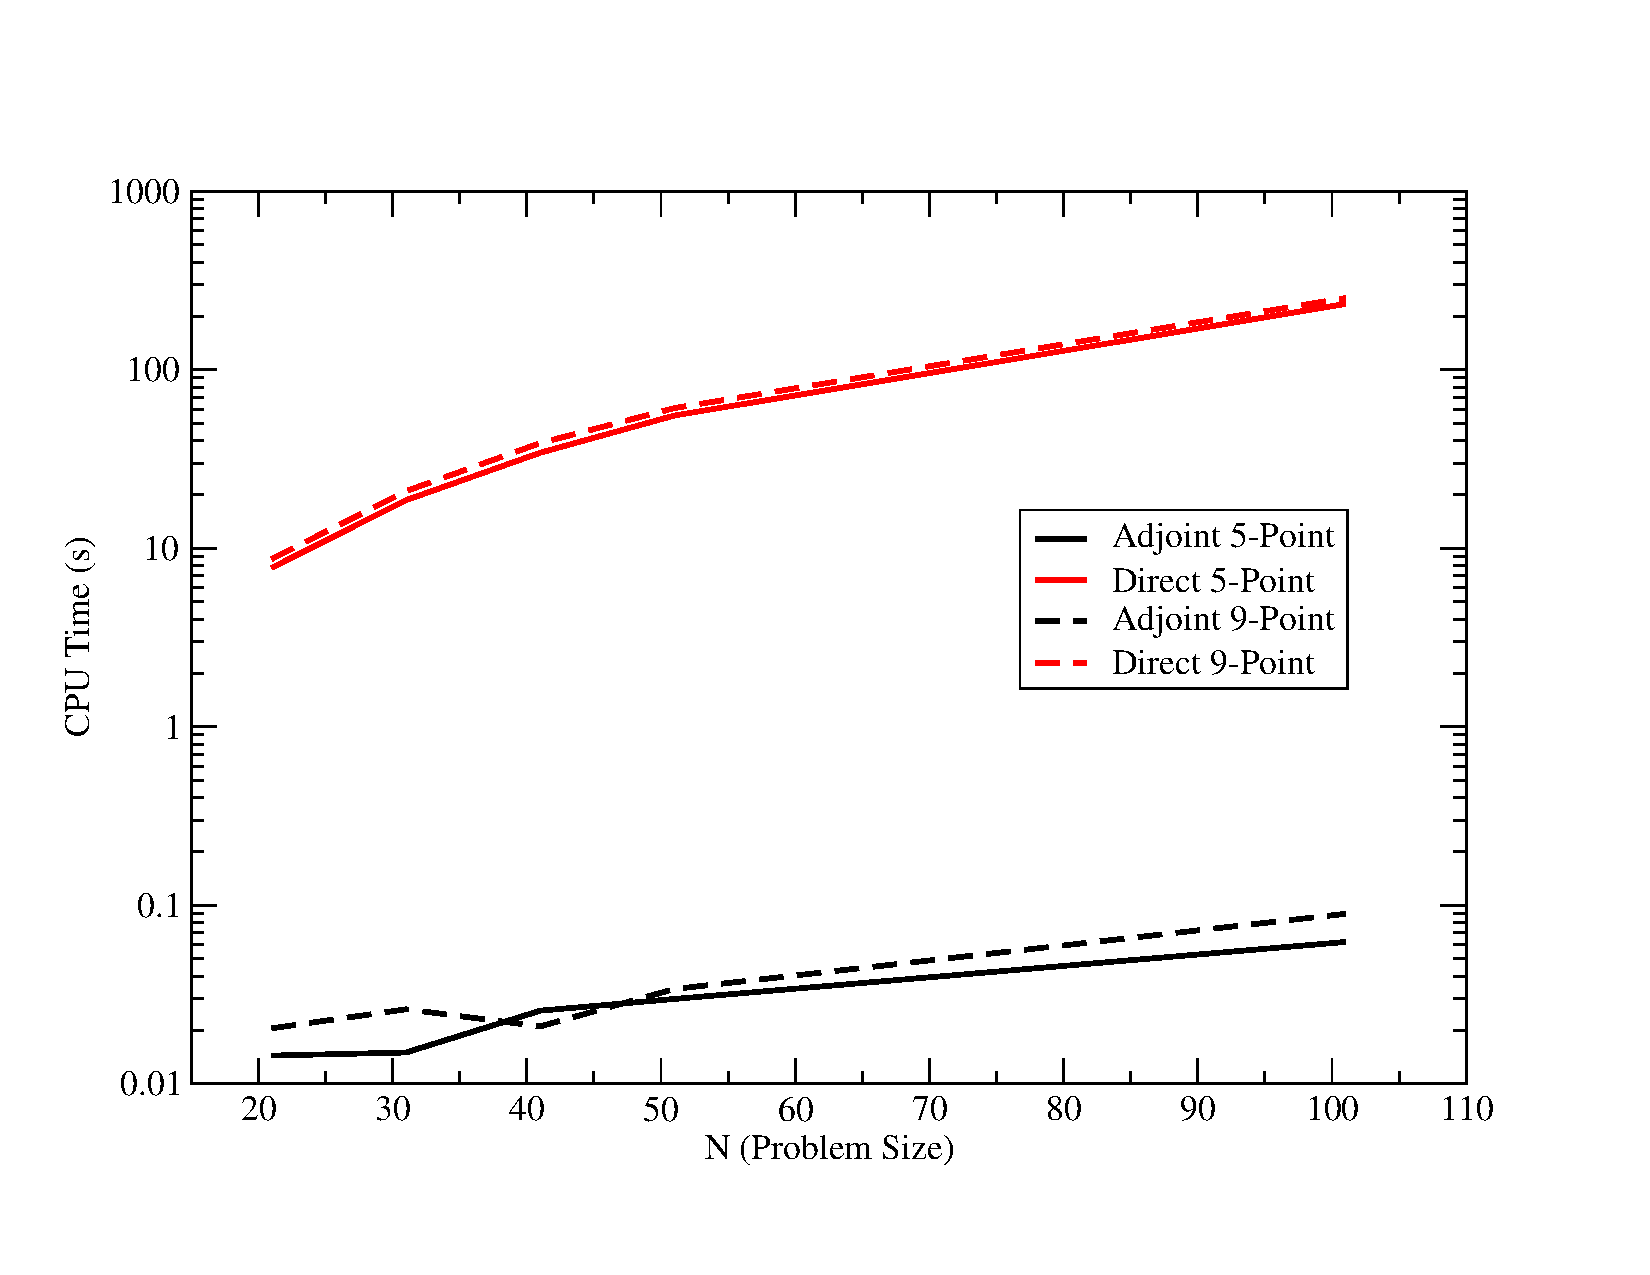
\includegraphics[width=5in,clip]{chapters/research_proposal/Adjoint_Direct_CPU_Time.pdf}
  \caption{\textbf{CPU Time (s) to converge vs. Problem Size ($N$ for
      an $N \times N$ square mesh).} \textit{Both the adjoint and
      direct solvers are used with the five point and nine point
      stencils. A significant CPU time speedup is noted with the
      adjoint method due to the reduced number of random walk
      events.}}
  \label{fig:poisson_cpu_time}
\end{figure}

\begin{figure}[h!]
  \centering
  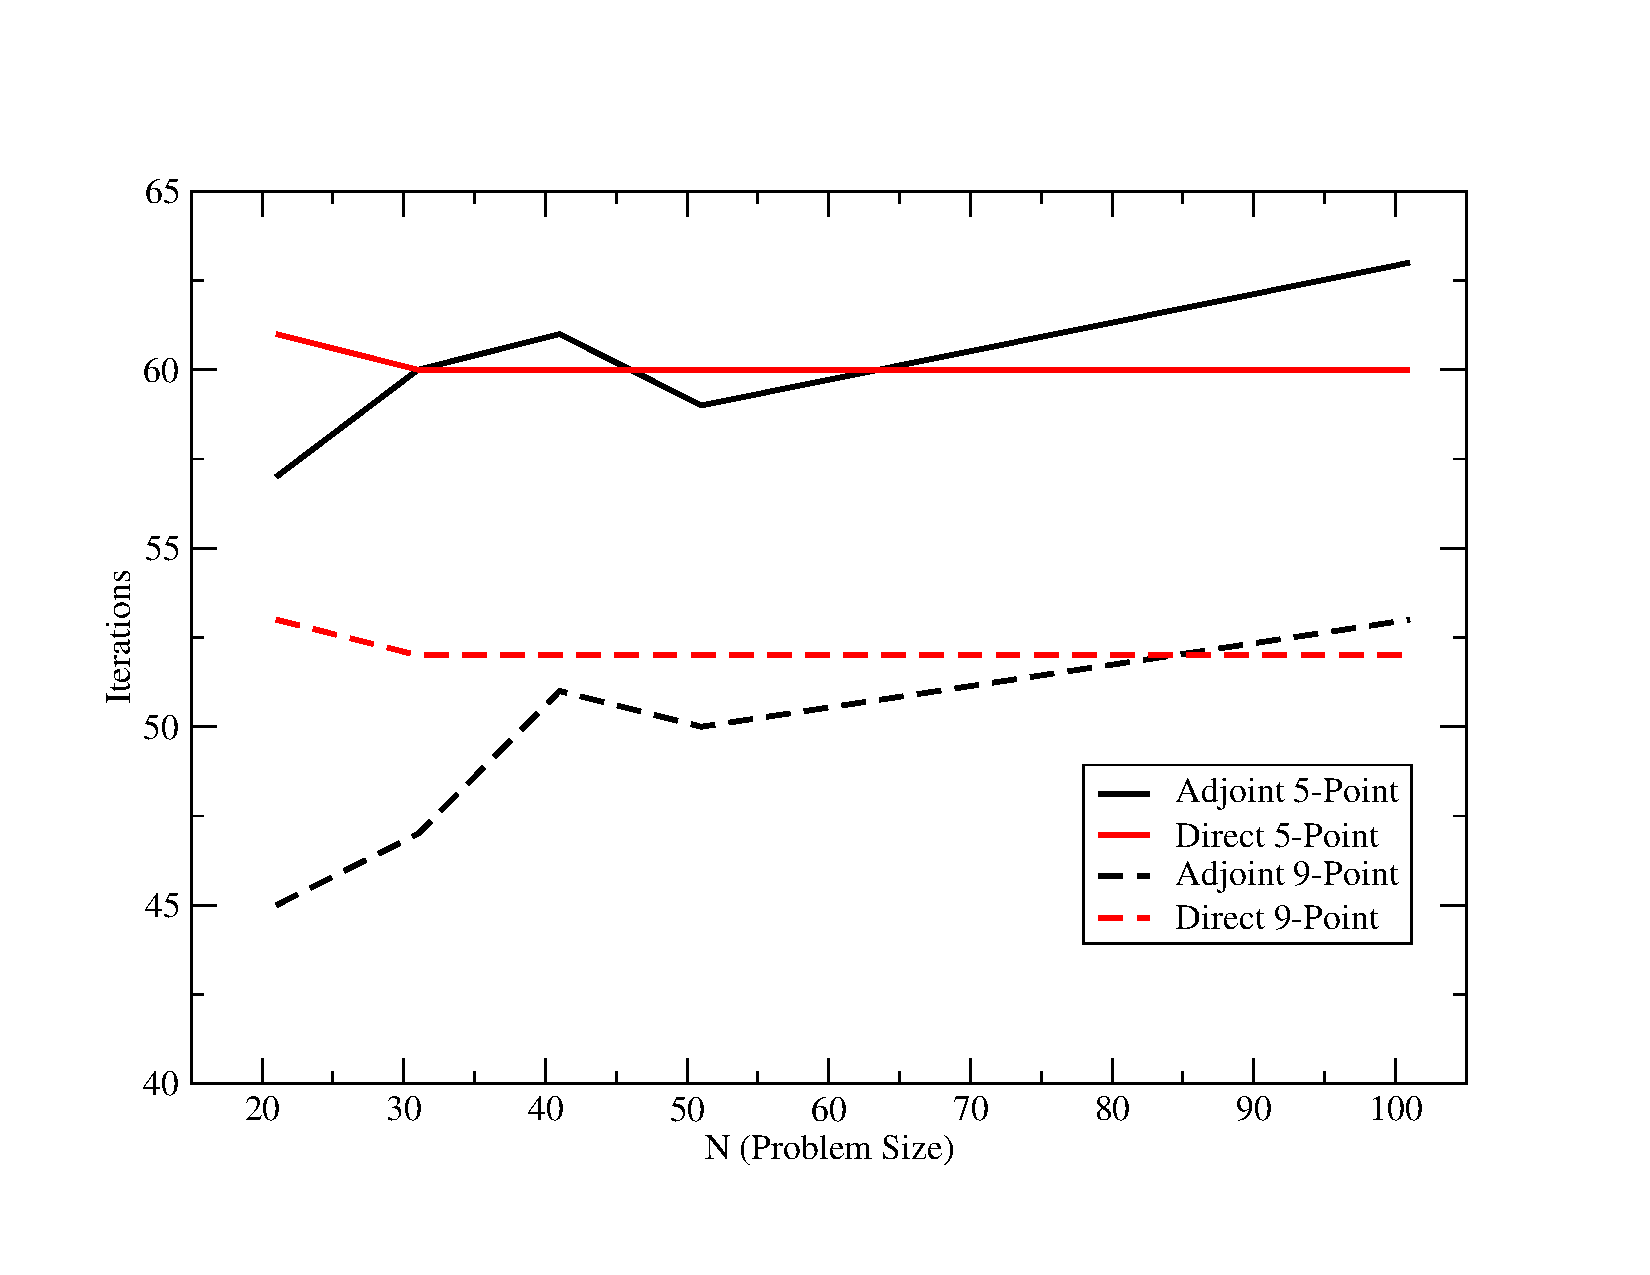
\includegraphics[width=5in,clip]{chapters/research_proposal/Adjoint_Direct_Iterations.pdf}
  \caption{\textbf{Iterations to converge vs. Problem Size ($N$ for an
      $N \times N$ square mesh).} \textit{Both the adjoint and direct
      solvers are used with the five-point and nine-point
      stencils. Both methods give similar iteration behavior.}}
  \label{fig:poisson_iterations}
\end{figure}

We see clearly in Fig.~\ref{fig:poisson_cpu_time} that the using the
adjoint solver with MCSA results in several orders of magnitude
speedup over the direct solver while the number of iterations required
to converge is of a similar scale. We expect this for several
reasons. First, with an equivalent number of histories specified for
both solvers and a system of size $N \times N$, the direct solver will
compute $N \times N$ random walks per permutation while the adjoint
solver will only compute one. This is necessary in the direct method
to ensure a contribution from each state as the random walk sequence
will only contribute to the starting state. For the adjoint method,
because the random walk sequence contributes to the state in which it
currently resides, fewer histories are neccessary to compute
contributions from all the nonzero parts of the source. Initially,
this may not seem like a fair comparison; however, we see from
Fig.~\ref{fig:poisson_iterations} that the number of iterations
required to converge is approximately the same and therefore the extra
computations performed by the direct method do not improve the error
estimation. Therefore, although the total number of random walks per
iteration is in fact larger for the direct method, the solution
computed at each iteration is no better than that computed by the
adjoint method.

As an additional comparison, the convergence behavior of MCSA can be
analyzed using both solvers to detect any performance benefits. To
assess the convergence properties of MCSA using each solver and
stencil, the infinity norm of the residual computed in
Eq.~(\ref{eq:mcsa}) was collected at each iteration for a fixed
problem size. Figure~\ref{fig:poisson_convergence} gives the results
of these computations. First, it is worthy to note on the semilog plot
that we are indeed achieving the expected exponential convergence from
MCSA. Second, we note that both the direct and adjoint methods have
approximately equivalent convergence behavior, leading to CPU time
being the dominating factor in method selection.
\begin{figure}[h!]
  \centering
  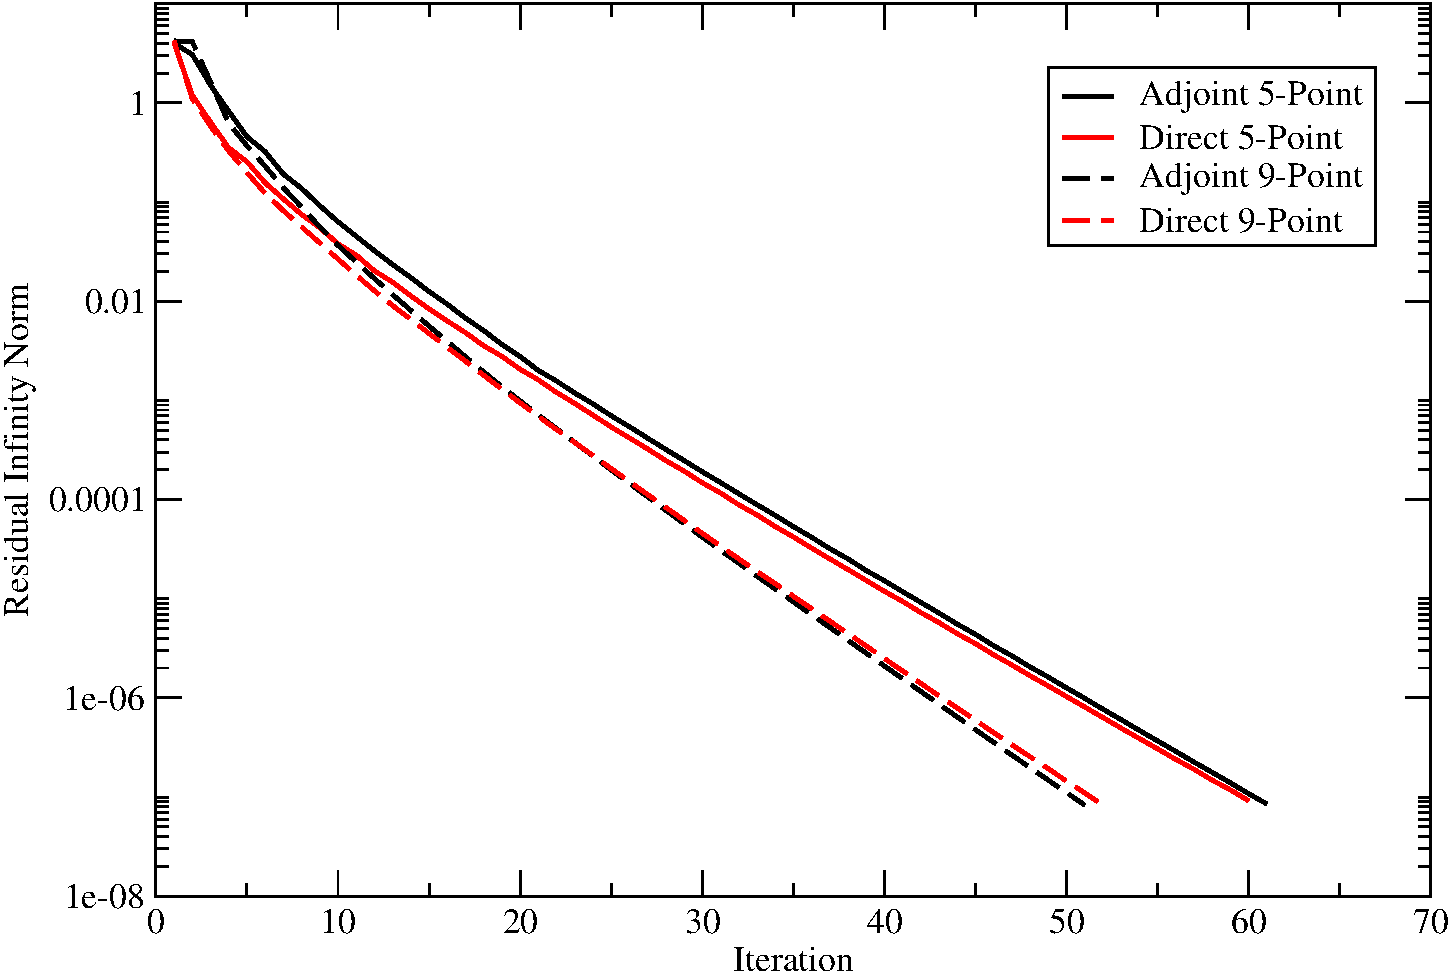
\includegraphics[width=5in,clip]{chapters/research_proposal/Adjoint_Direct_Convergence.pdf}
  \caption{\textbf{Infinity norm of the solution residual
      vs. iteration number for a problem of fixed size.} \textit{Both
      the adjoint and direct solvers are used with the five point and
      nine point stencils.}}
  \label{fig:poisson_convergence}
\end{figure}

\subsection{MCSA Application to Finite Element Problems}
\label{subsec:mcsa_finite_element}
The Epetra-based MCSA implementation has enabled the solution of
finite element problems leveraging the Panzer finite element assembly
engine, providing an initial basis for our experimental framework. To
demonstrate this, consider the 2-dimensional steady-state heat
equation:
\begin{equation}
  \boldsymbol{\nabla} \cdot k \boldsymbol{\nabla} T = Q\:,
  \label{eq:heat_equation}
\end{equation}
where $k$ is the thermal conductivity, $T$ is the temperature, and $Q$
is the thermal source. We can write the heat equation in weak form
using Eq~(\ref{eq:fe_weak_form}):
\begin{equation}
  \int_{\Omega} \boldsymbol{\nabla}^T \ve{v} k \boldsymbol{\nabla} T
  d\Omega - \int_{\Omega} \ve{v}Q d\Omega - \int_{\Gamma} \ve{v}
  \bar{q} d\Gamma - \int_{\Gamma} \ve{v} k \frac{\partial T}{\partial
    n} d\Gamma= 0\:,
  \label{eq:weak_heat_equation}
\end{equation}
where the boundary conditions have now been incorporated. We can
interpret the last two integral terms as the contributions from a
fixed boundary flux source and the flux through the domain
boundary. This weak formulation can then be directly implemented
within the finite element assembly engine along with the appropriate
boundary conditions and source terms. For this example, we choose a
square Cartesian grid with boundary conditions as shown in
Figure~\ref{fig:heat_eq_setup}.

\section{Stochastic Methods Verification}
\label{sec:method_verification}

\section{Numerical Experiments}
\label{sec:numerical_experiments}

\section{Challenge Problem}
\label{sec:challenge_problem}
